\documentclass[a4paper]{report}

\usepackage{NielsPackage}

\lstset{language=HTML}

\hypersetup{
	pdfauthor = {Niels Doorn},
	pdftitle = {JavaScript Game},
	pdfsubject = {HTML, CSS, JavaScript},
	pdfkeywords = {HTML,CSS,JavaScript,lesbrief},
	pdfcreator = {NielsDoorn/RocVanTwente}
}

\rhead{\textsc{JavaScript Game}}
\lhead{}
\chead{}
\lfoot{Niels Doorn, ROC van Twente \copyright~2012}
\cfoot{}
\rfoot{\thepage}

\fancypagestyle{plain}{
	\fancyhf{}
	\fancyfoot[L]{Niels Doorn, ROC van Twente \copyright~2012}
	\fancyfoot[C]{}
	\fancyfoot[R]{\thepage}
	\renewcommand{\headrulewidth}{0pt}
	\renewcommand{\footrulewidth}{0.4pt}
}

\begin{document}

\chapter*{\textcolor{seccol}{JavaScript} Game}
In deze lesbrief gaan we kijken hoe je de basis van een eenvoudig spel kunt maken in JavaScript.

\section*{Runway racer}
Voorbeeld van een eenvoudige basis voor een spel is het fantastische Runway Racer. Met JavaScript wordt er op een HTML canvas een achtergrond getekend en een raceauto. Door middel van de pijltjestoetsen kan de speler gas geven zodat de auto snelheid krijgt. Naar links en naar rechts sturen kan ook met de pijltjestoetsen. 

Als de auto sneller gaat, begint de auto ook te trillen. Meer `spel' elementen zitten er niet in. Om er echt een spel van te maken zou er bijvoorbeeld een computer gestuurde race-auto toegevoegd kunnen worden om er een wedstrijd van te maken, of het kan worden uitgebouwd tot een spel waarbij er objecten ontweken moeten worden.

\begin{center}
\resizebox{110mm}{!}{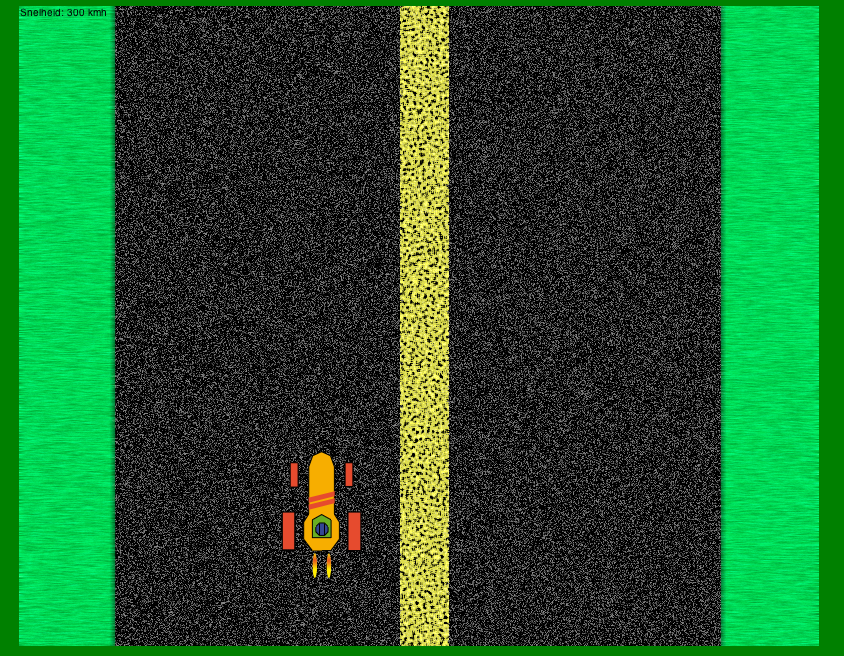
\includegraphics{runwayRacer}}
\end{center}

\section*{De opbouw van het spel}
Het spel bestaat uit HTML, CSS en JavaScript. Met name het JavaScript gedeelte is van belang voor het spel.

\subsection*{HTML}
In de HTML wordt net als in de vorige lesbrief een canvas tag gebruikt waar het spel op wordt getekend: 

\lstinputlisting{code/movingCar.html}

\subsection*{CSS Stylesheet}
\noindent De CSS stylesheet is ook hetzelfde als in de vorige lesbrief:

\lstinputlisting{code/style.css}

\subsection*{JavaScript}
\noindent Het grootste gedeelte van het spel is de JavaScript. We behandelen de belangrijkste functies per stuk, de (bijna) complete code volgt daarna. Dat is de code inclusief de initialisatie functie en declaratie van variabelen et cetera.

\subsubsection*{Animatie loop}
Voor actiespellen zoals dit is het belangrijk dat het scherm steeds opnieuw wordt opgebouwd, optimaal is het als dit met 60fps wordt gedaan. Het is afhankelijk van wat er allemaal moet gebeuren binnen het spel en de kracht van de computer of dat aantal van 60fps wordt gehaald. 

In de JavaScript code zorgt de \textbf{requestAnimationFrame} functie hiervoor. Om er voor te zorgen dat dit in alle browsers werkt moet je gebruik maken van prefixes. Het belangrijkste stukje code is de \textbf{animLoop} functie, die wordt 60 keer per seconde aangeroepen en roept zelf weer de \textbf{draw} functie aan die het scherm op gaat bouwen:

\begin{lstlisting}[numbers=none]
// animatie
// vraag aan de browser om maximaal 60 fps te animeren
window.requestAnimFrame = (function(callback){
	return window.requestAnimationFrame ||
	window.webkitRequestAnimationFrame ||
	window.mozRequestAnimationFrame ||
	window.oRequestAnimationFrame ||
	window.msRequestAnimationFrame ||
	function(callback){
		window.setTimeout(callback, 1000 / 60);
	};
})();

(function animloop(){
	requestAnimFrame(animloop);
	draw();
})();
\end{lstlisting}

\noindent De \textbf{animLoop} functie zorgt voor de animatie loop. Het belangrijkste wat in ons geval moet gebeuren is het tekenen van het scherm. De \textbf{draw} functie zorgt hiervoor. 

\subsubsection*{De schermopbouw tekenen}

De \textbf{draw} functie zorgt ervoor dat het scherm leeg wordt gemaakt met de \textbf{clearRect} functie, daarna wordt de \textbf{drawBackground} die de achtergrond laat zien. De snelheid van de auto wordt in het scherm geschreven met de \textbf{fillText} functie.

Als dit is gebeurd wordt de auto getekend. De auto kan op scherm naar links en rechts bewegen, dit doen we door de context te \emph{transleren} naar de juiste positie met de \textbf{ctx.translate} aanroep. Transleren is een ander woord voor verschuiven. Je verschuift de context naar een nieuwe uitgangspositie waar je wilt gaan tekenen.

Door te transleren is het eenvoudiger om de auto te tekenen, de coordinaten bij het tekenen blijven dan altijd hetzelfde en hoeven niet opnieuw berekend te worden.

Op deze manier kunnen we ook roteren en transformeren. Voor dat we transleren, roteren of transformeren is het belangrijk om de context op te slaan om er voor te zorgen dat hetgene wat we al hebben getekend niet mee verschuift of draait. Dit doen we met de \textbf{ctx.save} functie.

Als we de auto hebben getekend op het canvas roepen we tot slot een stukje `artificial intelligence' aan om de auto wat te laten trillen als hij sneller gaat.

\begin{lstlisting}[numbers=none]
// het tekenen van het scherm
function draw() {
	var ctx = canvas.getContext("2d");
 	// canvas leeg maken, het canvas is 800px breed en 640px hoog
	ctx.clearRect(0, 0, 800, 640);
 	// teken de bewegende achtergrond
	drawBackground(ctx);
	// schrijf snelheid op het scherm omgerekend naar km/h op het canvas
	ctx.fillText("Snelheid: " + Math.round(speed * (300/40)) + " kmh", 1, 10);
  	// bewaar deze situatie
	ctx.save();
	// transleer de context, zodat de auto op de juiste plaats wordt getekend
	ctx.translate(x, y);
	// teken de auto
	drawCar(ctx);
	// artificial intelligence aanroepen (trillen van de auto)
	ai();
}
\end{lstlisting}

\subsubsection*{De achtergrond}
Om het idee te geven dat de auto aan het rijden is, verplaatsen we de auto niet maar wordt de achtergrond verschoven. De afbeelding die moet dus hoger zijn dan de hoogte van het canvas. Bijvoorbeeld twee keer zo hoog. Meer mag ook om te voorkomen dat het opvalt dat er steeds dezelfde weg voorbij komt. 

Om de achtergrond te herhalen moeten we bijhouden hoever we de achtergrond hebben verschoven. Als er niet verder geschoven kan worden beginnen we opnieuw. Als de auto sneller gaat, moet de achtergrond sneller scrollen, daarom wordt de variabele \emph{speed} gebruikt om de verschuiving te bepalen.

Deze manier werkt, zij het met meerdere achtergronden, goed bij platform spellen zoals Mario.

\begin{lstlisting}[numbers=none]
// bewegende achtergrond tekenen
// de afbeelding van de auto is 1280px hoog,
// iedere keer wordt het plaatje verschoven,
// en als helemaal tot bovenaan is verschoven 
// opnieuw getekend
function drawBackground(ctx) {
	ctx.drawImage(bgImage,0 ,bgOffset);
    bgOffset += speed / 2;
    if (bgOffset > 0) {
	  bgOffset = -640;
    }
}
\end{lstlisting}

\subsubsection*{Besturing met het toetsenbord}
Om de auto sneller te laten rijden kan het toetsenbord gebruikt worden. Iedere keer als er een toets wordt ingedrukt wordt er in de \textbf{handleKeyboardInput} functie gekeken of er een van de pijltjestoetsen is ingedrukt. Als dat het geval is, wordt de bijbehorende functie aangeroepen, bijvoorbeeld up in het geval van het pijltje omhoog.

De manier waarop dit gebeurt heet een \textbf{switch}. Dit lijkt op een \textbf{if} functie maar is in sommige gevallen, waarbij er vele mogelijkheden zijn handiger en overzichtelijker. Vergeet bij iedere \textbf{case} niet af te sluiten met een \textbf{break}, anders wordt niet alleen de code van de huidige case uitgevoerd, maar ook de code van de opvolgende case totdat er een break gevonden wordt.

Andere toetsenbordcodes voor bijvoorbeeld spatie et cetera kun je o.a. hier vinden: \url{http://goo.gl/8F6zS}.

\begin{lstlisting}[numbers=none]
// pijltjes toetsen
function handleKeyboardInput(evt) {
    evt = evt || window.event;
    switch (evt.keyCode) {
		case 37:		// pijltje links
			left();
			break;		// break niet vergeten!
		case 38:		// pijltje omhoog
			up();
			break;	
		case 39:		// pijltje rechts
			right();
			break;
		case 40:		// pijltje omlaag
			down();
			break;		
    }
}
\end{lstlisting}

\subsubsection*{De gehele code}
Naast de functies die hierboven staan zijn er nog de variabelen declaraties, de init functie en het tekenen van de auto. Hieronder de complete listing van runway racer, op het tekenen van de auto na. Het tekenen van de auto gebeurd door de bekende commando's op het canvas zoals ook in de vorige lesbrief te lezen is.
\lstinputlisting{code/script-stripped.js}

\clearpage

\section*{Opdrachten}

\noindent \textbf{Opdracht 1:} Maak je eigen `spel'
Maak een begin van een eigen spel dat ook gebruik maakt van een canvas en van de gameloop zoals in dit spel. Bedenk eerst wat voor spel je wilt maken, maak schetsen en beschrijf wat je wilt maken. Laat je idee en schetsen aan je docent zien ter goedkeuring.

Je kunt denken aan een platform spel, een racespel of aan een ander soort spel.

Maak daarna alle vector tekeningen, bitmaps en html en css. Schrijf vervolgens de JavaScript code. Test alles goed voor je het inleverd!
\\

\noindent \textbf{Opdracht 2:} Maak de webpagina af
Maak een mooie website van je spel, alleen het canvas is zo kaal.

\section*{Beoordeling}
De uitwerkingen van deze opdrachten inclusief schetsen en beschrijving van je game moeten worden ingeleverd. Je krijgt hiervoor een cijfer.

\end{document}